\section{Разработка и применение метода анализа локальной вариабельности при помощи построения подграфов}
Работа выполнена совместно с Конановым Дмитрием Николаевичем.\\


\subsection{Проблема сравнительного анализа расположения генов в большом наборе геномов.}

Визуализация блоков синтении часто применяется для сравнения генного состава оперонов, островов патогенности либо других областей генома, интересующих исследователя. Такой способ визуализации нагляден и хорошо подходит для небольшого количества геномов. Но сравнение нескольких десятков последовательностей затруднительно, а нескольких сотен --- практически невозможно. При этом, количество прочитанных геномов быстро растет, для многих видов их уже доступно несколько сотни и даже тысяч. Анализ геномов в подобных масштабах требует новых подходов. Мы предлагаем в качестве такого подхода графовое представление порядка расположения генов в геномах. Выше мы описали применение графового представления для численной оценки локальной вариабельности геномов. Ниже мы опишем применение графового представления для визуализации изменений в небольших фрагментах генома. 

\subsection{Алгоритм поиска подграфа для анализа участка генома}

Визуализация полного графа набора геномов допустима в случае небольших геномов, характерных для вирусов, но не в случае бактерий --- полный граф будет слишком велик для эффективной визуализации. Для бактериальных геномов имеет смысл проводить анализ подграфа - части полного графа, соответствующей некоторому региону интереса (например, оперону).

Для построения подграфа мы реализовали следующий набор действий. Вначале, выбирается референсный геном и указывается начало и конец анализируемой области. Затем, строится граф, содержащий цепочку узлов референсного генома и к нему добавляются узлы, представленные в других геномах и связанные с референсной цепочкой. Добавление узлов происходит пока путь снова не вернется в референсную цепочку, либо пока не будет достигнут предел на длину (параметр \textit{tails}). Алгоритм для построения подграфа можно представить следующим псевдокодом:
\begin{enumerate} 
\item Вход: graph (граф группы геномов)
\item Параметры: \textit{reference (референсный геном), start\_node (начало анализируемого фрагмента), end\_node (конец анализируемого фрагмента), max\_depth (ограничение на длину обходных путей), tails (ограничение на длину свободный путей), minimal\_edge\_weight (минимальный вес ребра)}.
\item Результат: subgraph (подграф интересующего фрагмента генома)
\item subgraph $\leftarrow$ пустой граф
\item target\_chain $\leftarrow$ цепочка узлов из референсного генома между start\_node и end\_node
\item добавить target\_chain в subgraph
\item deviating\_paths $\leftarrow$ найти все пути начинающиеся и заканчивающиеся в target\_chain
\item для каждого пути path из deviating\_paths выполнить
\item если длина path < \textit{max\_depth} то
\item  \quad  добавить path в subgraph
\item иначе
\item \quad path\_tails  $\leftarrow$ начальный и конечный фрагмент path длиной \textit{tails}
\item \quad	добавить path\_tails в subgraph
\item для каждого ребра edge из subgraph выполнить
\item \quad если вес edge < \textit{minimal\_edge\_weight} то
\item \quad \quad удалить edge из subgraph
\item удалить области связанности subgraph не связанные с target\_chain
\item вернуть subgraph
\end{enumerate}

Данный алгоритм, реализованный на языке Python3, доступен в репозитории: \url{https://github.com/DNKonanov/gene_graph_lib}

В приведенном выше алгоритме предусмотрено два фильтра, которые помогают уменьшать размер подграфа, если он оказывается слишком велик.  Даже при рассмотрении небольшого участка генома, соответствующий ему подграф может содержать длинные пути, например, из-за крупных хромосомных перестроек в рассматриваемых геномах. Для того, чтобы эти длинные пути не затрудняли визуализацию и последующий анализ, в алгоритме предусмотрен фильтр, который заменяет длинный путь его начальным и концевым фрагментом ("усами"). Максимальная длина пути, который будет показан полностью, задается параметром \textit{max\_depth}, размер фрагментов, которые сохраняются вместо длинного пути (длина "усов") задается параметром \textit{tails} (рисунок~\ref{img:tails_schema}). Пути которые начинаются либо заканчиваются, но не начинаются и заканчиваются, в рассматриваемой области ("уходящие" за пределы рассматриваемой области) также сокращаются до фрагментов длиной \textit{tails}.

\begin{figure}[!ht] 
  \center
  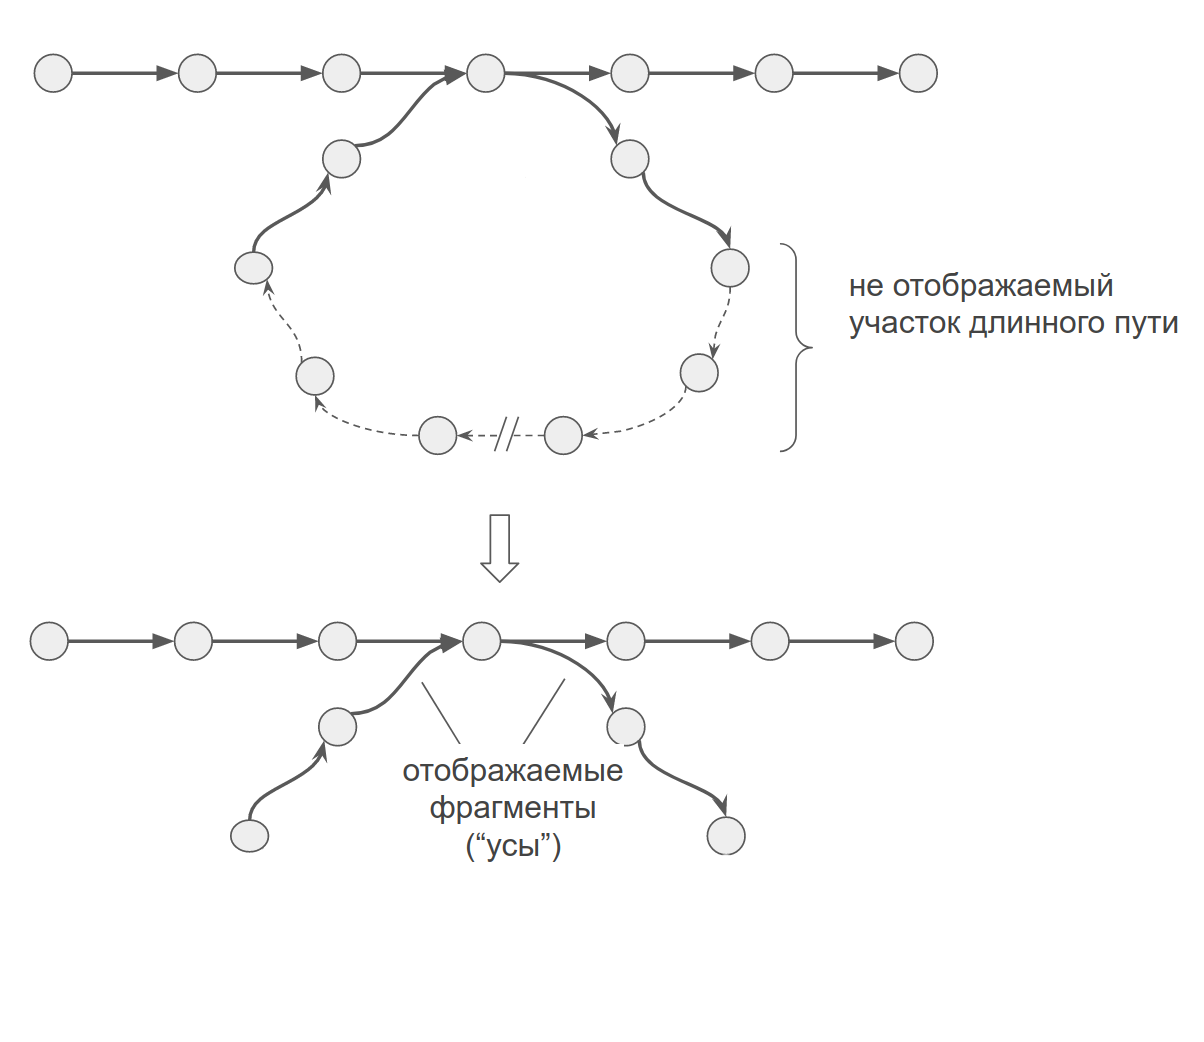
\includegraphics[width=0.8\textwidth]{Dissertation/images/subgraphs/tails_schema_v2.png}
  \caption{Схематическая иллюстрация работы фильтра длинных путей. }
  \label{img:tails_schema} 
\end{figure}

Еще один фильтр позволяет не включать в подграф ребра с маленьким весом, то есть те, которые встречаются в малом количестве геномов. За это отвечает параметр \textit{minimal\_edge\_weight}. Применение фильтров особенно важно при анализе "горячих" точек изменчивости.

%############################################################# SUBGRAPHS
\section{Примеры применения представления порядка чередования генов в виде графа.}

В работе \cite{rakitina2017genome}, были установлены опероны, которые статистически значимо чаще (метод определения будет описан ниже) встречались у изолятов \textit{E. coli} полученных от пациентов с воспалительным заболеванием кишечника --- болезнью Крона, по отношению к изолятам от здоровых людей. Носительство данных оперонов, вероятно, выгодно при нахождении бактерий в условиях воспалительной реакции со стороны организма хозяина, а может и провоцирует воспаление. Метод для поиска оперонов, различающих группы бактерий, будет описан ниже.

Рассмотрим, как выглядят подграфы, соответствующие оперонам, чья встречаемость оказалась выше в изолятах, полученных от пациентов с болезнью Крона, по сравнению с комменсальными штаммами. На этих примерах будут проиллюстрированы основные моменты анализа графового представления фрагментов генома. 

\textbf{Опероны утилизации гемина и пропандиола}

На рисунках~\ref{img:sub_hem} и ~\ref{img:sub_pdu} показаны графы, построенные в окрестностях оперонов захвата гемина (hemin uptake, hmu) и утилизации пропандиола (propanediol utilization operon, pdu), соответственно. В качестве референсного генома нами был взят геном \textit{Escherichia coli LF82}, в анализ были включены 327 финишированных геномов доступных в базе RefSeq. Для построения данных графов мы использовали следующие параметры: \textit{tails} = 1, \textit{max\_depth} = 30, \textit{minimal\_edge\_weight} = 5. 

Рассмотрим для начала более простой случай оперона захвата гемина. Данный оперона состоит из следующих генов: транспортный белок (Hemin transport protein HemS), АТФ-связывающий белок захвата гемина (Hemin import ATP-binding protein HmuV), гемин-связывающий периплазматический белок (hemin-binding periplasmic protein HmuT), кислороднезависимый копропорфириноген-III оксидазоподобный белок (oxygen-independent coproporphyrinogen-III oxidase-like protein) и два гипотетических белка (здесь и далее мы приводим аннотации последовательностей, полученные при помощи утилиты prokka \cite{seemann2014prokka}).

Как видно из графа, представленного на рисунке~\ref{img:sub_hem}, данный оперон расположен в консервативном генном контексте: слева расположен регулятор транскрипции HTH-типа, справа --- гипотетический белок. Дуговое ребро обходящее оперон сверху говорит о том, что в некотором наборе геномов данный оперон отсутствует и других вариантов генов у них в этом локусе не наблюдается. 

\begin{figure}[!ht] 
  \center
  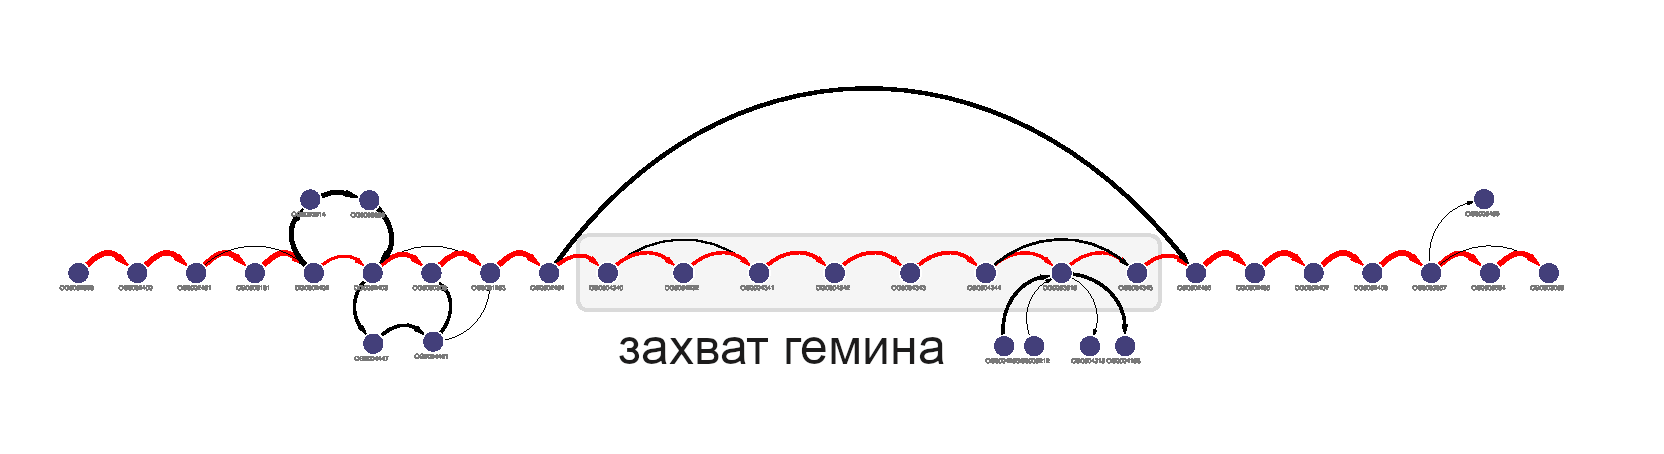
\includegraphics[width=0.8\textwidth]{Dissertation/images/subgraphs/hemin.png}
  \caption{Граф представляющий окрестность оперона утилизации гемина (hemin uptake, hmu).}
  \label{img:sub_hem} 
\end{figure}

В оперон утилизации пропандиола (propanediol utilization operon, pdu) входят гены, кодирующие: белок утилизации пропандиола PduU, малая субъединица пропандиол-дегидратазы, белок утилизации пропандиола PduB, белок с механизмом концентрации углекислого газа CcmK, субъединица альфа-фактора реактивации диолдегидратазы, белок утилизации пропандиола PduV, альдегид-алкоголь дегидрогеназа, C-диамид аденозил трансфераза ириновой кислоты Cob I, большая субъединица  пропандиол дегидратазы, фосфат-пропаноил трансфераза, альдегид-алкоголь дегидрогеназа. Как видно из рисунка~\ref{img:sub_pdu} наблюдается консервативность контекста расположения pdu оперона у тех штаммов, в которых он представлен: слева от него расположен ген, кодирующий белок CobU  (участвует в синтезе витамина B12), справа --- гипотетический белок. Ребро обходящее оперон (дуга ниже оперона) говорит о том, что в ряде штаммов в данном контексте нет иных вариантов генов. Наблюдается некоторая вариабельность внутри оперона, соответствующая нескольким вариантам данного оперона \cite{rakitina2017genome}. Помимо pdu оперона, в том же контексте, у ряда штаммов наблюдается альтернативный набор генов (узлы и ребра, расположенные выше оперона), в который входят гены транспорта железа (FepC, FcuA, HmuU), гены мобильных элементов (retroviral integrase core domain, transposase DDE Tnp ISL3) и множество гипотетических генов с неизвестной функцией. Примечательна вариабельность этого альтернативного набора генов. Вероятно, данный участок генома часто служит местом рекомбинационных событий, приводящих к изменению набора генов, причем эти изменения не имеют строгого начала и конца (не сайт специфичны), но часто накладываются друг на друга. 

\begin{figure}[!ht] 
  \center
    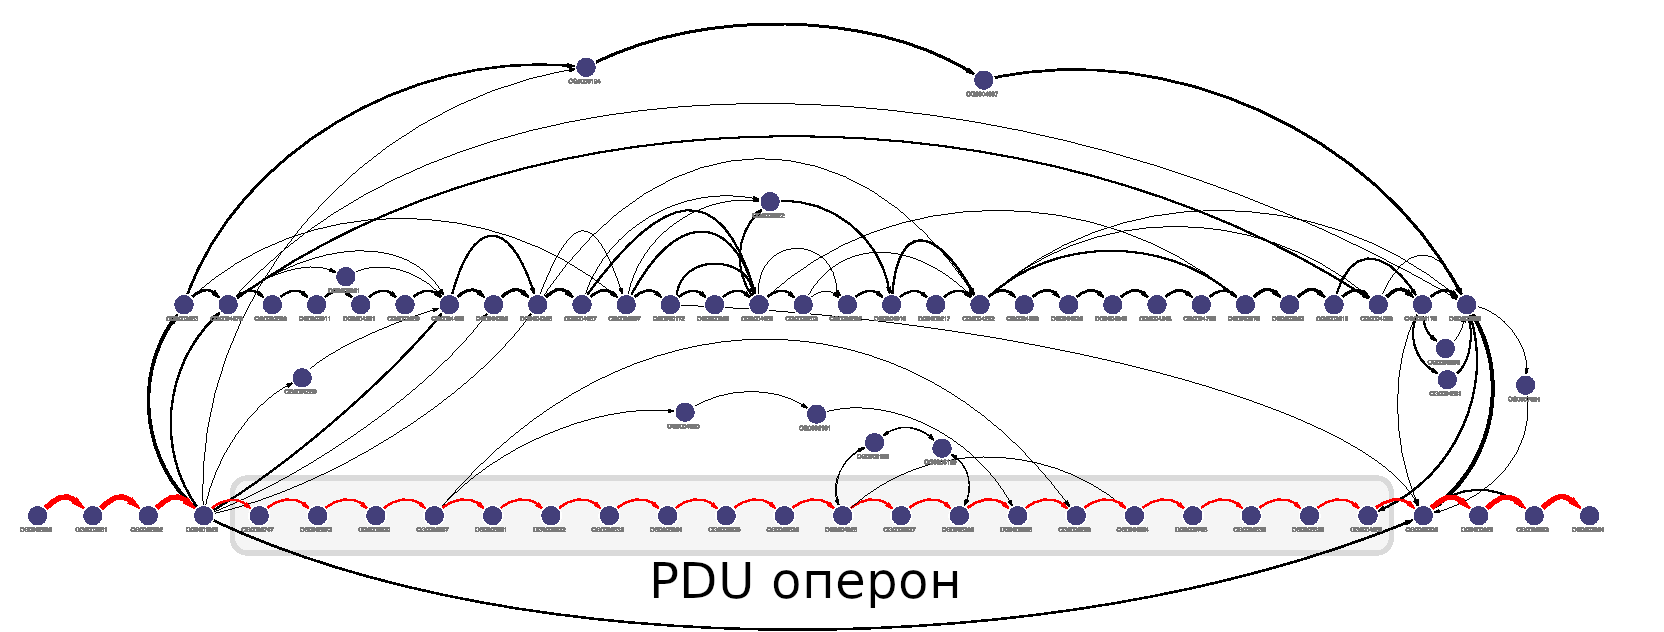
\includegraphics[width=0.8\textwidth]{Dissertation/images/subgraphs/pdu_laconic.png}
  \caption{Граф представляющий окрестность оперона утилизации пропандиола (propanediol utilization operon, pdu). }
  \label{img:sub_pdu} 
\end{figure}

Если рассмотреть более длинный фрагмент генома вблизи pdu оперона  (рисунок~\ref{img:pdu_wide}), видно расположенный рядом еще более вариабельный участок. Примечательно, что в нем не содержится аннотированных генов связанных с мобильностью ДНК, вместо этого присутствуют гены синтеза капсулы и многочисленные гипотетические гены с неизвестной функцией. 

\begin{figure}[!ht] 
  \center
    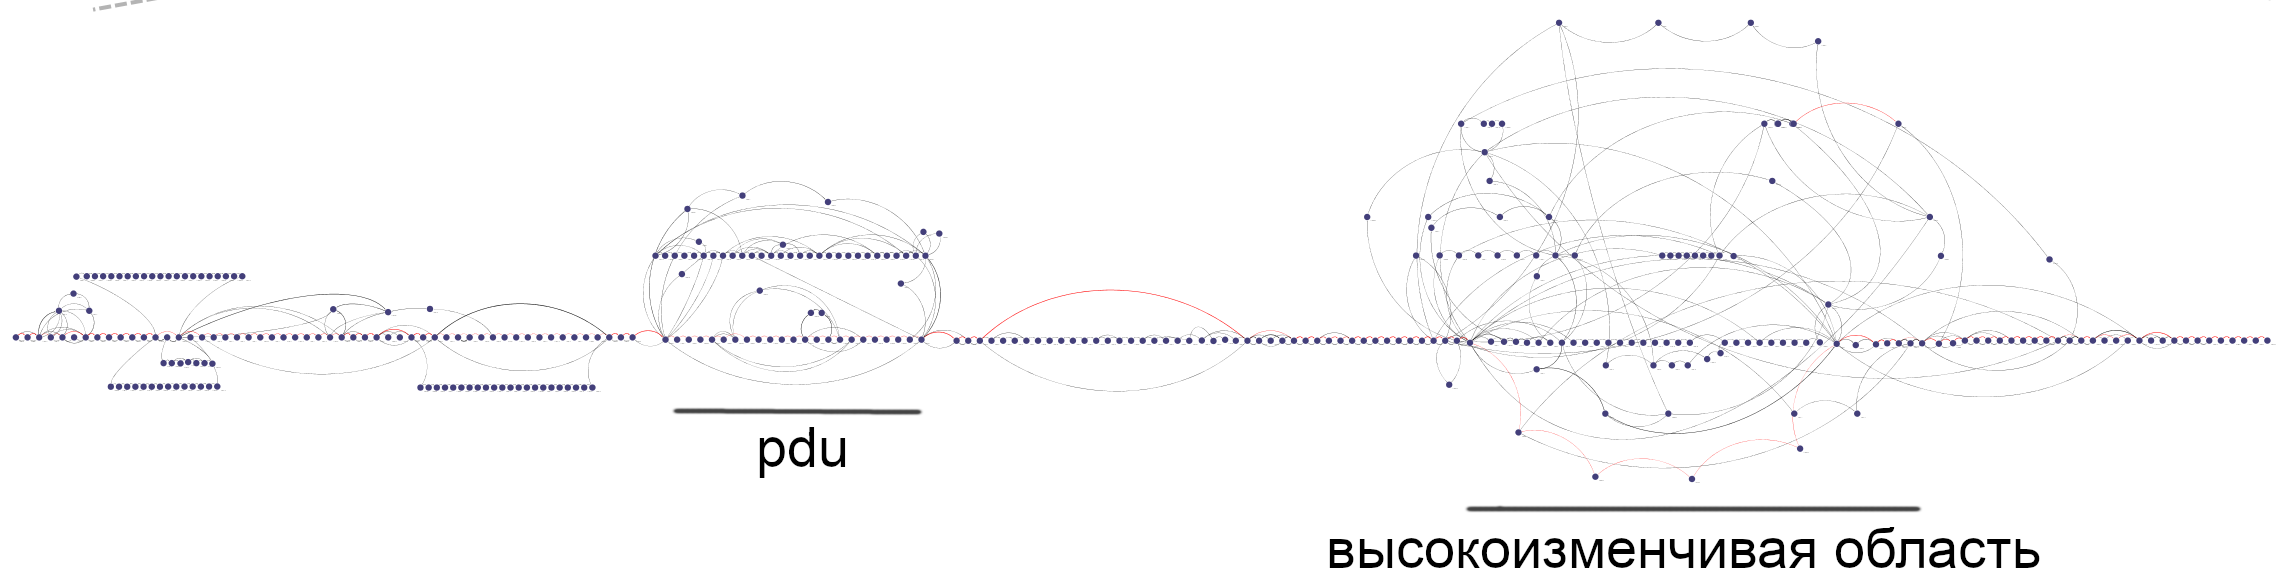
\includegraphics[width=\textwidth]{Dissertation/images/subgraphs/subgraph_largest.png}
  \caption{Граф представляющий окрестность оперона утилизации пропандиола (propanediol utilization operon, pdu). }
  \label{img:pdu_wide} 
\end{figure}

\textbf{Кластер генов синтеза бактериальной капсулы}

\begin{figure}[!ht] 
  \center
    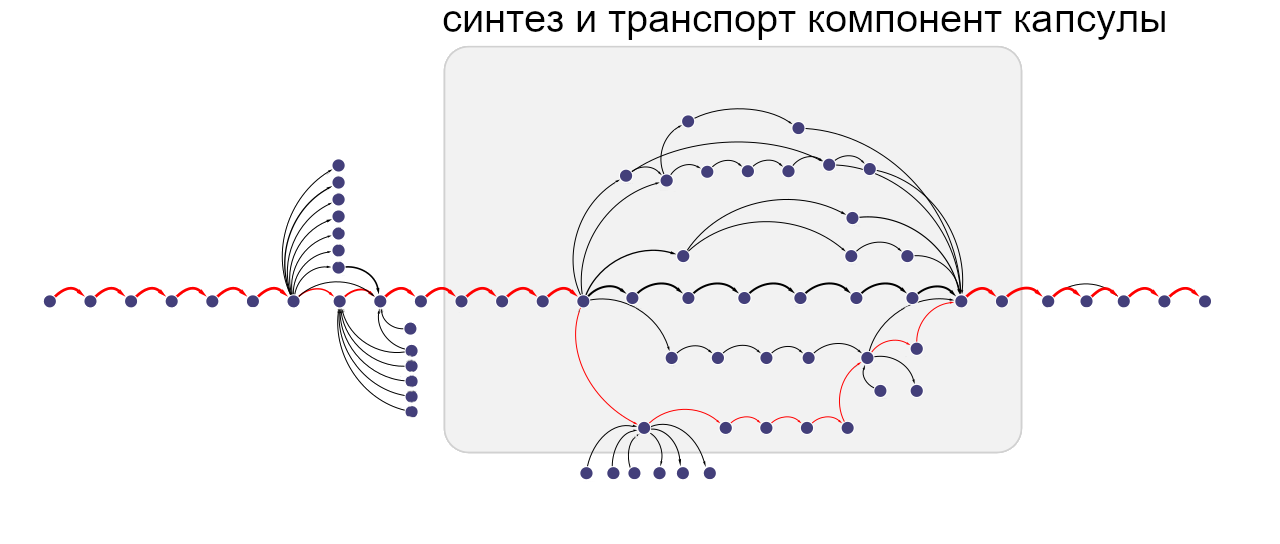
\includegraphics[width=\textwidth]{Dissertation/images/subgraphs/capsular_subgraph.png}
  \caption{Граф представляющий окрестность кластера генов синтеза бактериальной капсулы. }
  \label{img:capsule_sub_small} 
\end{figure}

На рисунке~\ref{img:capsule_sub_small} показано графовое представление окрестности оперона синтеза бактериальной капсулы. 
Видно, что оперон состоит из консервативных фрагментов, фланкирующих вариабельный участок. Вариабельная часть оперона соответствует генам, отвечающим за синтез серотип-специфичного набора полимеров капсулы и кодирующим: глицерин-3-фосфат цитидилилтрансферазу, синтазу N,N'-диацетиллегионаминовой кислоты, N-ацилнейраминат цитидилилтрансферазу, белок биосинтеза полисиаловой кислоты P7, O-ацетилтрансферазу полисиаловой кислоты, ацетилтрансферазу EpsM, гликозилтрансфераза EpsJ, глицерол-фосфат трансферазу тейхоевой кислоты, поли (глицеролфосфат) полимеразу тейхоевой кислоты, поли (рибитол-фосфат) полимеразу тейхоевой кислоты, рибитол-фосфат-полимеразу тейхоевой кислоты TarL, UDP-галактопиранозную мутазу, UDP-Glc альфа-D-GlcNAc-дифосфоундекапренол бета-1,3-глюкозилтрансфераза WfgD, UDP-глюкозо-4-эпимеразу, вирджиниамицин А ацетилтрансферазу. Гены консервативной части кодируют белки, участвующие в транспорте синтезированных веществ через клеточную стенку: транспортный белок полисиаловой кислоты KpsD, 3-дезокси-манно-октулосонат цитидилилтрансферазу, транспортный белок полисиаловой кислоты KpsM, транспортный АТФ-связывающий белок полисиаловой кислоты KpsT \cite{clarke1999genetic}. В референесном штамме \textit{LF82} в вариабельную часть входят гены синтеза тейхоевых кислот. 

Фрагменты единичной длины, расположенные слева от оперона, говорят о том, что есть много путей, которые не попадают в построенный подграф поскольку либо слишком длинные, либо заканчиваются вне отображаемой области и поэтому были сокращены до коротких фрагментов (параметр \textit{tails} при анализе был равен 1). Если расширить рассматриваемую область, то многие из этих путей станут видны (рисунок~\ref{img:capsule_sub_large}, данный граф получен с параметрами: \textit{tails} = 1, \textit{minimal\_edge} = 2). Вид данного графа говорит о значительной вариабельности участка генома, содержащего гены синтеза капсулы.

\begin{figure}[!ht] 
  \center
    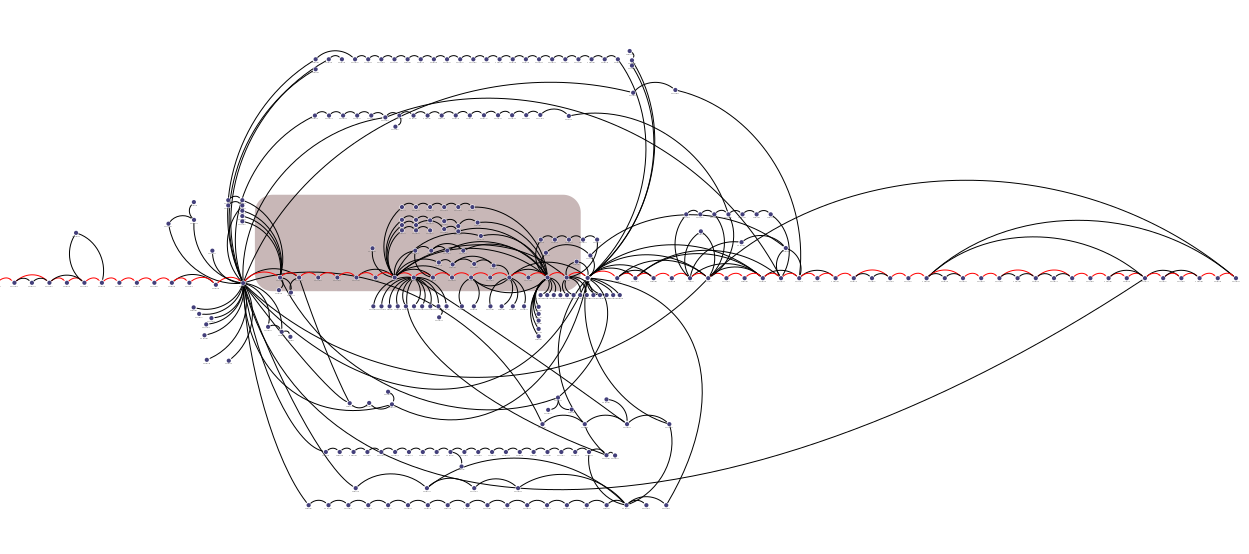
\includegraphics[width=\textwidth]{Dissertation/images/subgraphs/capsular_subgraph2_red.png}
  \caption{Граф представляющий расширенную окрестность генов синтеза бактериальной капсулы (отмечены областью красного цвета). }
  \label{img:capsule_sub_large} 
\end{figure}

Вариабельность состава капсулы адаптивна (это помогает бактериям избегать распознавание иммунной системой организма-хозяина либо бактериофагами \cite{cress2014masquerading, lukavcova2008role}. Можно предположить, что для бактерии выгодно такая локализация этих генов, где изменения могут происходить чаще. Можно выдвинуть гипотезу, что данный участок генома обладает некоторыми (еще не установленными) свойствами, которые обеспечивают значительную вариабельность генного состава, и в том числе - вариабельность состава генов капсулы.

\textbf{Оперон метаболизма глиоксилата}

На рисунке~\ref{img:glioxilate} показан граф отражающий область генома в окрестности оперона метаболизма глиоксилата. Данный оперон является частью геномного острова, включающего в себя четыре оперона: три оперона метаболизма углеводов и глицерина (ptn, cgl и gcx) и один оперон инвазии ibe. Данный остров описан у вызывающего менингит штамма \textit{Escherichia coli K1}, и, методом экспериментального мутагенеза, показан как функционально значимый для проявления ее патогенных свойств \cite{huang2001novel}. 

\begin{figure}[!ht] 
  \center
    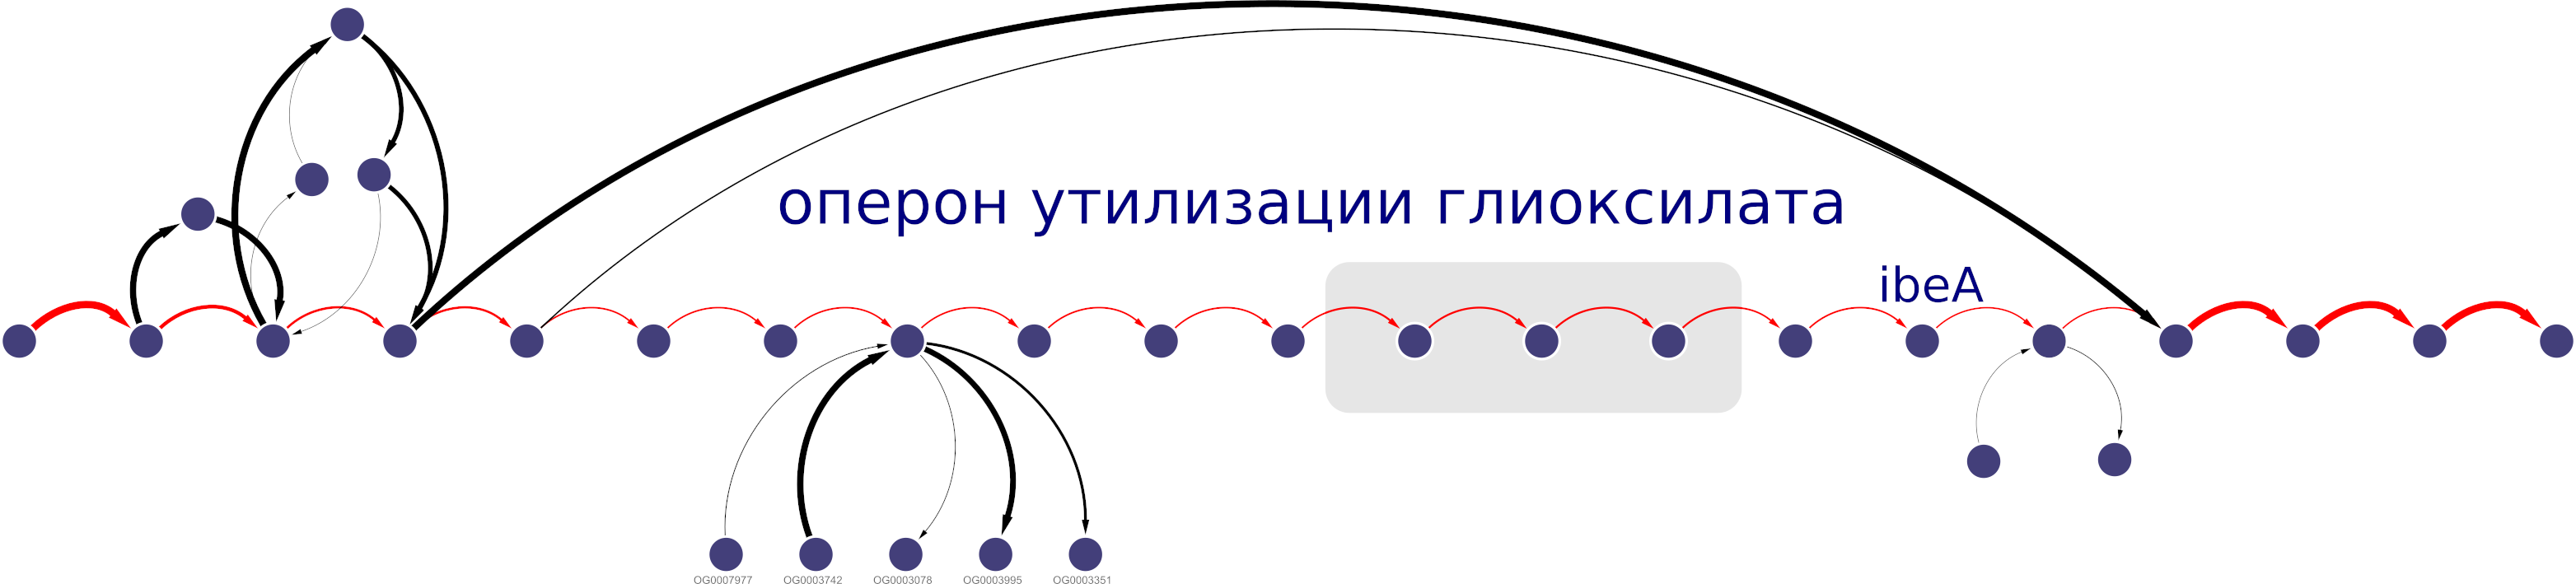
\includegraphics[width=\textwidth]{Dissertation/images/subgraphs/glyoxilate_metabolism_operon_crop.png}
  \caption{Граф представляющий окрестность генов оперона метаболизма глиоксилата. }
  \label{img:glioxilate} 
\end{figure}

% Замечание: мелко! продумать рисунки

Интересно, что хотя мы наблюдали значительную вариабельность геномных островов у \textit{E. coli} и других бактериальных видов, в данном случае наблюдается весьма низкая вариабельность генного состава: остров либо представлен у некоторых организмов, либо - нет, и в последнем случае, на его месте не обнаруживаются какие-либо вставки.

\textbf{Оперон захвата и утилизации сорбозы}

Данный оперон содержит следующие гены, кодирующие: транскриптационный регулятор оперона, сорбитол дегидрогеназу, фосфоенолпируват-зависимую сахарную фосфотрансферазу EII и дигидроантикапсин-7-дегидрогеназу.

В случае данного оперона наблюдается картина, схожая с опероном захвата гемина и глиоксилата: оперон либо присутствует у части штаммов, либо нет, без выраженной изменчивости геномов в данном регионе (рисунок~\ref{img:sorbitol}). 

\begin{figure}[!ht] 
	\center
	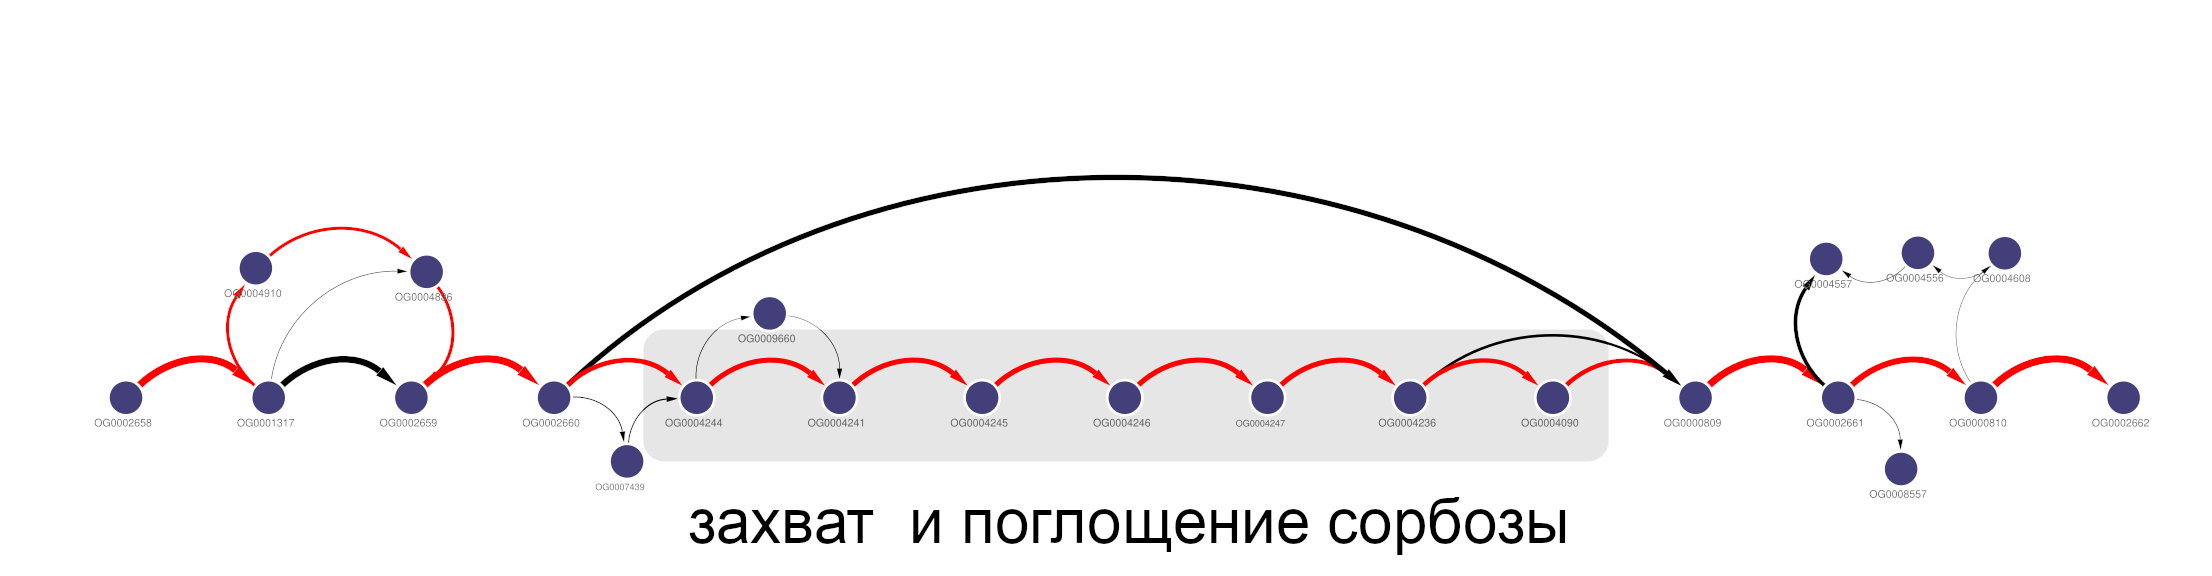
\includegraphics[width=\textwidth]{Dissertation/images/subgraphs/sorbitol.png}
	\caption{Граф представляющий окрестность генов оперона захвата и утилизации сорбозы. }
	\label{img:sorbitol} 
\end{figure}

%Добавить: последний граф для профага и обобщение
